\documentclass[11pt]{article}

\usepackage[spanish]{babel}
\usepackage[margin=1in]{geometry}
\usepackage{amsmath, amssymb, amsfonts}
\usepackage{booktabs}
\usepackage{tabularx}
\usepackage{enumitem}
\usepackage{tcolorbox}
\usepackage{hyperref}
\usepackage{listings}
\usepackage{xcolor}
\usepackage{parskip}
\usepackage{csquotes}
\usepackage{pgfplots}
\usepackage[backend=biber,style=numeric,sorting=none]{biblatex}
\addbibresource{referencias.bib}

\usetikzlibrary{arrows.meta}
\pgfplotsset{compat=1.18}

% Long identifiers (tool_names, notifications/initialized) inside \texttt
% don't hyphenate by default and overflow narrow table columns — this lets
% them break at underscores/slashes instead of causing overfull hboxes.
\newcommand{\code}[1]{\texttt{\seqsplit{#1}}}
\usepackage{seqsplit}

\lstset{
  language=bash,
  basicstyle=\ttfamily\footnotesize,
  breaklines=true,
  columns=flexible,
  keepspaces=true,
  commentstyle=\color{gray}\itshape,
  keywordstyle=\color{blue!70!black}\bfseries,
  stringstyle=\color{green!40!black},
  frame=L,
  xleftmargin=2em,
  showstringspaces=false,
  tabsize=4
}

\lstdefinelanguage{yaml}{
  keywords={},
  sensitive=false,
  comment=[l]{\#},
  morestring=[b]',
  morestring=[b]"
}

\title{\textbf{Data Catalog MCP: Servidor MCP de Catálogo de Datos con Validación de Calidad} \vspace{1em}\\
  Redes de Computadoras - CC3067}
\author{José Antonio Mérida Castejón}
\date{\today}

\begin{document}

\maketitle

\section{Especificación del servidor MCP}

\subsection{Caso de uso}
El servidor implementa un catálogo de datos interno con validación de
calidad, dirigido al equipo de analítica de una empresa mediana. El
problema que atiende es común en organizaciones que acumulan datasets de
distintas fuentes (exportaciones de CRM, ventas, recursos humanos) sin
documentación centralizada: los analistas invierten tiempo considerable en
determinar qué datos existen, qué significa cada columna, en qué unidades
está expresada, y si un extracto recibido cumple las condiciones mínimas de
calidad antes de usarlo. El servidor expone herramientas de solo lectura y
sin estado que el chatbot anfitrión coordina en lenguaje natural; el LLM
coordina las llamadas e interpreta los resultados, pero no genera
información por su cuenta.

El escenario concreto se enmarca como \textbf{Meridian Holdings}, una
empresa ficticia con cuatro unidades de negocio (Meridian Mobile, Meridian
Retail, Meridian Commerce y Recursos Humanos corporativos), cada una con su
propio sistema de origen. El patrón corresponde a herramientas de uso
industrial ya establecido --- los archivos \code{schema.yml} de dbt, las
suites de expectativas de Great Expectations, y catálogos de datos como
DataHub o Amundsen --- sin constituir un \emph{feature store}, ya que no
calcula ni sirve valores de \emph{features} para inferencia.

\subsection{Origen de la información}
El servidor obtiene su información de dos fuentes complementarias, ambas
locales al servidor y sin dependencias externas en tiempo de consulta:

\begin{enumerate}
  \item \textbf{Archivos de datos en formato Parquet} (\code{data/*.parquet}),
  sobre los cuales se calculan estadísticas y validaciones. Cinco datasets:
  suscriptores de Meridian Mobile, ventas de Meridian Retail, transacciones
  de comercio electrónico de Meridian Commerce, rotación de personal de RR.HH.,
  y un extracto mensual sin validar (copia de suscriptores con inconsistencias
  introducidas de forma controlada y reproducible, para demostrar
  \code{validate\_dataset}).
  \item \textbf{Catálogo declarativo} en un archivo YAML (\code{catalog.yaml}),
  escrito manualmente, que actúa simultáneamente como diccionario de datos y
  definición de reglas de calidad. Para cada columna se declara su tipo,
  descripción, unidad y las reglas que debe cumplir:

\begin{lstlisting}[language=yaml]
- name: customerID
  type: string
  description: Unique customer identifier
  unit: null
  rules:
    - not_null
    - unique
    - regex: '^\d{4}-[A-Z]{5}$'
      severity: error
\end{lstlisting}
\end{enumerate}

Las reglas de calidad operan a nivel de columna (\code{not\_null},
\code{unique}, \code{range}, \code{allowed\_values}, \code{regex},
\code{type\_check}) o a nivel de dataset (\code{row\_count},
\code{freshness}). Cada regla declara una severidad: \code{error} invalida
el dataset para uso posterior; \code{warning} señala una anomalía que
amerita revisión sin bloquear el flujo de trabajo.

\subsection{Arquitectura interna}
El servidor (\code{cmd/server}) está escrito en Go, sin SDKs de MCP ni
librerías de JSON-RPC de terceros --- todo el framing de mensajes y el
manejo del protocolo se implementó a mano, según lo exigido por el
enunciado. Los paquetes relevantes:

\begin{itemize}
  \item \code{internal/jsonrpc} --- framing JSON-RPC 2.0 sobre un
  \code{io.Reader}/\code{io.Writer} genérico: lee mensajes delimitados por
  línea, los decodifica a la estructura \code{Message} (\code{jsonrpc},
  \code{id}, \code{method}, \code{params}, \code{result}, \code{error}), y
  distingue solicitud de notificación según la presencia del campo
  \code{id}.
  \item \code{internal/mcp} --- implementa el ciclo de vida MCP sobre esa
  capa: \code{initialize}, \code{notifications/initialized},
  \code{tools/list} y \code{tools/call}, más el despacho a cada
  herramienta (un archivo \code{tool\_*.go} por herramienta).
  \item \code{internal/catalog} --- parseo de \code{catalog.yaml} a
  estructuras tipadas.
  \item \code{internal/data} --- resuelve cada entrada del catálogo al
  archivo Parquet correspondiente y lo lee.
  \item \code{internal/embeddings} --- cliente de embeddings con dos
  proveedores intercambiables (Ollama local, Gemini remoto) para
  \code{search\_catalog}.
  \item \code{internal/config} --- configuración vía variables de entorno
  (\code{TRANSPORT}, \code{CATALOG\_PATH}, \code{DATA\_DIR}, \code{PORT}, etc.).
\end{itemize}

Esta separación permite que la \emph{misma} implementación se ejecute sin
modificaciones tanto de forma local (stdio) como remota (HTTP/Cloud Run):
el núcleo MCP es agnóstico al transporte.

\subsection{Herramientas expuestas (endpoints MCP)}
Todas las herramientas se invocan mediante el método JSON-RPC
\code{tools/call}, identificadas por su campo \code{name} y con argumentos
en \code{params.arguments}. La Tabla~\ref{tab:tools} detalla parámetros y
tipo de retorno de cada una.

\begin{table}[h]
\centering
\begin{tabularx}{\textwidth}{@{}l X@{}}
\toprule
\textbf{Herramienta} & \textbf{Parámetros y descripción} \\
\midrule
\code{ping} & Sin parámetros. Retorna \code{"pong"}; verificación de salud. \\
\code{list\_datasets} & Sin parámetros. Retorna nombre, descripción, origen,
  número de filas y fecha de actualización de cada dataset registrado. \\
\code{describe\_dataset} & \code{dataset} (string, requerido). Retorna el
  diccionario de datos completo: columnas, tipos, descripciones, unidades y
  reglas declaradas. \\
\code{profile\_column} & \code{dataset}, \code{column} (string, requeridos).
  Retorna estadísticas según el tipo: cuantiles y atípicos para numéricas,
  cardinalidad y valores frecuentes para categóricas, rango y vacíos para
  fechas. \\
\code{validate\_dataset} & \code{dataset} (string, requerido). Ejecuta las
  reglas declaradas contra los datos reales; retorna veredicto general
  (reglas evaluadas/aprobadas/fallidas), detalle por regla con severidad y
  porcentaje de violaciones, y hasta cinco valores de ejemplo por violación. \\
\code{find\_undocumented\_columns} & \code{dataset} (string, requerido).
  Compara las columnas presentes en el Parquet contra las declaradas en el
  catálogo, para detectar documentación desactualizada. \\
\code{search\_catalog} & \code{query} (string, requerido). Búsqueda
  semántica (embeddings, similitud coseno) o por palabra clave si el
  servicio de embeddings no está disponible. Consulta dos índices
  independientes --- datasets y columnas --- y retorna ambos conjuntos por
  separado, ya que sus puntajes no son comparables entre sí. \\
\code{chart\_column} & \code{dataset}, \code{column} (requeridos). Genera un
  histograma, gráfica de barras o serie de tiempo según el tipo de columna,
  y lo retorna como bloque de contenido tipo imagen del protocolo MCP. \\
\bottomrule
\end{tabularx}
\caption{Herramientas expuestas por el servidor MCP y sus parámetros.}
\label{tab:tools}
\end{table}

\subsection{Búsqueda semántica en dos niveles}
\code{search\_catalog} construye al iniciar el servidor dos índices
vectoriales: uno de datasets (nombre, descripción, origen) para consultas
de granularidad amplia, y otro de columnas (nombre y descripción de la
columna junto con la descripción de su dataset, ya que el nombre de una
columna por sí solo suele ser demasiado breve para una representación
vectorial informativa). La recuperación es por similitud coseno mediante
multiplicación matricial; dado el tamaño reducido del índice ($\approx$100
vectores), una búsqueda exhaustiva es apropiada y no se justifica una base
de datos vectorial dedicada.

\subsection{Privacidad y servicios externos}
La generación de embeddings se delega a un servicio externo (Ollama local o
Gemini), lo que evita incorporar un modelo local al contenedor y mantiene
una imagen ligera con arranques en frío reducidos. El servidor transmite a
ese servicio \textbf{únicamente metadatos} --- nombres de dataset, nombres
de columna, descripciones y unidades, redactados manualmente en el
catálogo --- y las consultas del usuario, nunca registros ni valores de
los archivos de datos. Esta separación es una decisión de diseño
deliberada que hace viable el caso de uso en un entorno donde los datos
suelen estar sujetos a restricciones contractuales o regulatorias.

\subsection{Transporte y despliegue}
\begin{itemize}
  \item \textbf{stdio} (local): mensajes JSON delimitados por línea sobre
  stdin/stdout del proceso hijo, spawneado por el anfitrión (\code{cmd/host}
  o \code{cmd/client}) según \code{client.json}.
  \item \textbf{HTTP} (remoto): un único endpoint (\code{POST /}) que recibe
  un objeto JSON-RPC por solicitud y responde con el resultado
  correspondiente. Se activa con \code{TRANSPORT=http}; el puerto se toma
  de la variable \code{PORT} inyectada por la plataforma.
\end{itemize}

El servidor remoto se desplegó en \textbf{Google Cloud Run}, construido
mediante Cloud Build directamente desde el repositorio de GitHub (sin
necesidad de Docker local): una imagen \code{distroless} de dos etapas
(compilación Go, luego binario estático más \code{catalog/} y
\code{data/*.parquet}). Las credenciales de embeddings (\code{EMBEDDINGS\_API\_KEY})
se inyectan vía Secret Manager, nunca como variable de entorno en texto
plano. Ambos transportes exponen exactamente los mismos métodos MCP:
\code{initialize}, \code{tools/list} y \code{tools/call}, por lo que el
anfitrión usa el servidor remoto de forma idéntica al local, solo cambiando
la entrada \code{url} por \code{command} en \code{client.json}.

\section{Análisis de la comunicación (Wireshark)}

Se realizaron dos capturas complementarias contra el mismo servidor MCP
(mismo binario, mismo código, mismos mensajes JSON-RPC), diferenciadas
únicamente por el transporte:

\begin{itemize}
  \item \textbf{Captura remota}: el anfitrión conectado al servidor
  desplegado en Google Cloud Run
  (\code{data-catalog-mcp-53268160127.northamerica-\allowbreak
  south1.run.app}) sobre HTTPS. Filtrada en Wireshark con
  \code{ipv6.addr == 2600:1900:4243:200::}. Al ser HTTPS, el contenido de
  aplicación viaja cifrado; esta captura se usa para el análisis de las
  capas de enlace, red y transporte (\S\ref{sec:capas}), incluyendo el
  handshake TCP y TLS reales contra el servidor en la nube.
  \item \textbf{Captura local}: el mismo anfitrión conectado al mismo
  servidor ejecutándose localmente con \code{TRANSPORT=http} (sin TLS),
  filtrada con \code{tcp.port == 8091}. Dado que el formato y contenido de
  los mensajes JSON-RPC es idéntico independientemente del transporte, esta
  captura se usa para inspeccionar y clasificar los mensajes JSON-RPC en
  texto plano (\S\ref{sec:jsonrpc}), lo cual no es posible directamente
  sobre la captura remota sin descifrar la sesión TLS.
\end{itemize}

\subsection{Mensajes JSON-RPC capturados}
\label{sec:jsonrpc}
Se identifican tres tipos de mensaje JSON-RPC en la especificación:
\textbf{solicitud} (\code{request}, contiene \code{id} y \code{method}),
\textbf{respuesta} (\code{response}, contiene \code{id} y \code{result} o
\code{error}), y \textbf{notificación} (\code{notification}, sin \code{id},
no espera respuesta --- usada por MCP para \code{notifications/initialized}).
Estos mensajes de sincronización (\code{initialize} /
\code{notifications/initialized}) son los que establecen el protocolo antes
de que el anfitrión pueda invocar herramientas; el resto son solicitud/respuesta
ordinarias de operación.

% TODO: completar la tabla con los mensajes reales capturados en la sesión
% local (número de frame de Wireshark, id JSON-RPC, etc.) y agregar las
% figuras local-03..08 referenciadas abajo una vez tomadas las capturas.
\begin{table}[h]
\centering
\begin{tabularx}{\textwidth}{@{}l l l X@{}}
\toprule
\textbf{\#} & \textbf{Tipo} & \textbf{Método} & \textbf{Observaciones} \\
\midrule
1 & Solicitud & \code{initialize} & Handshake inicial, negocia \code{protocolVersion} y \code{capabilities}. \\
2 & Respuesta & --- & Responde al \code{id} de (1) con las capacidades del servidor. \\
3 & Notificación & \code{notifications/initialized} & Sin \code{id}; confirma que el cliente completó el handshake. \\
4 & Solicitud & \code{tools/list} & Pide el catálogo de herramientas disponibles. \\
5 & Respuesta & --- & Responde con el arreglo \code{tools} (Tabla~\ref{tab:tools}). \\
6 & Solicitud & \code{tools/call} & Ej. \code{list\_datasets}, sin argumentos. \\
7 & Respuesta & --- & \code{content} con el resultado en texto. \\
\bottomrule
\end{tabularx}
\caption{Clasificación de los mensajes JSON-RPC observados en la captura.}
\label{tab:jsonrpc}
\end{table}

% TODO: capturas pendientes (contra el servidor local con TRANSPORT=http,
% filtro tcp.port == 8091). Guardar en docs/figs/ con estos nombres exactos
% y descomentar el bloque de figuras correspondiente:
%
%   local-01-filtered-list.png     lista de paquetes con el filtro aplicado
%   local-02-loopback-header.png   encabezado "Null/Loopback" (sin Ethernet real)
%   local-03-http-stream.png       Follow > HTTP Stream, conversación completa
%   local-04-initialize-request.png   cuerpo JSON de la solicitud initialize
%   local-05-initialize-response.png  cuerpo JSON de la respuesta a initialize
%   local-06-notification.png         notifications/initialized (sin "id")
%   local-07-toolscall-request.png    cuerpo JSON de una solicitud tools/call
%   local-08-toolscall-response.png   cuerpo JSON de su respuesta
%
% \begin{figure}[ht]
% \centering
% 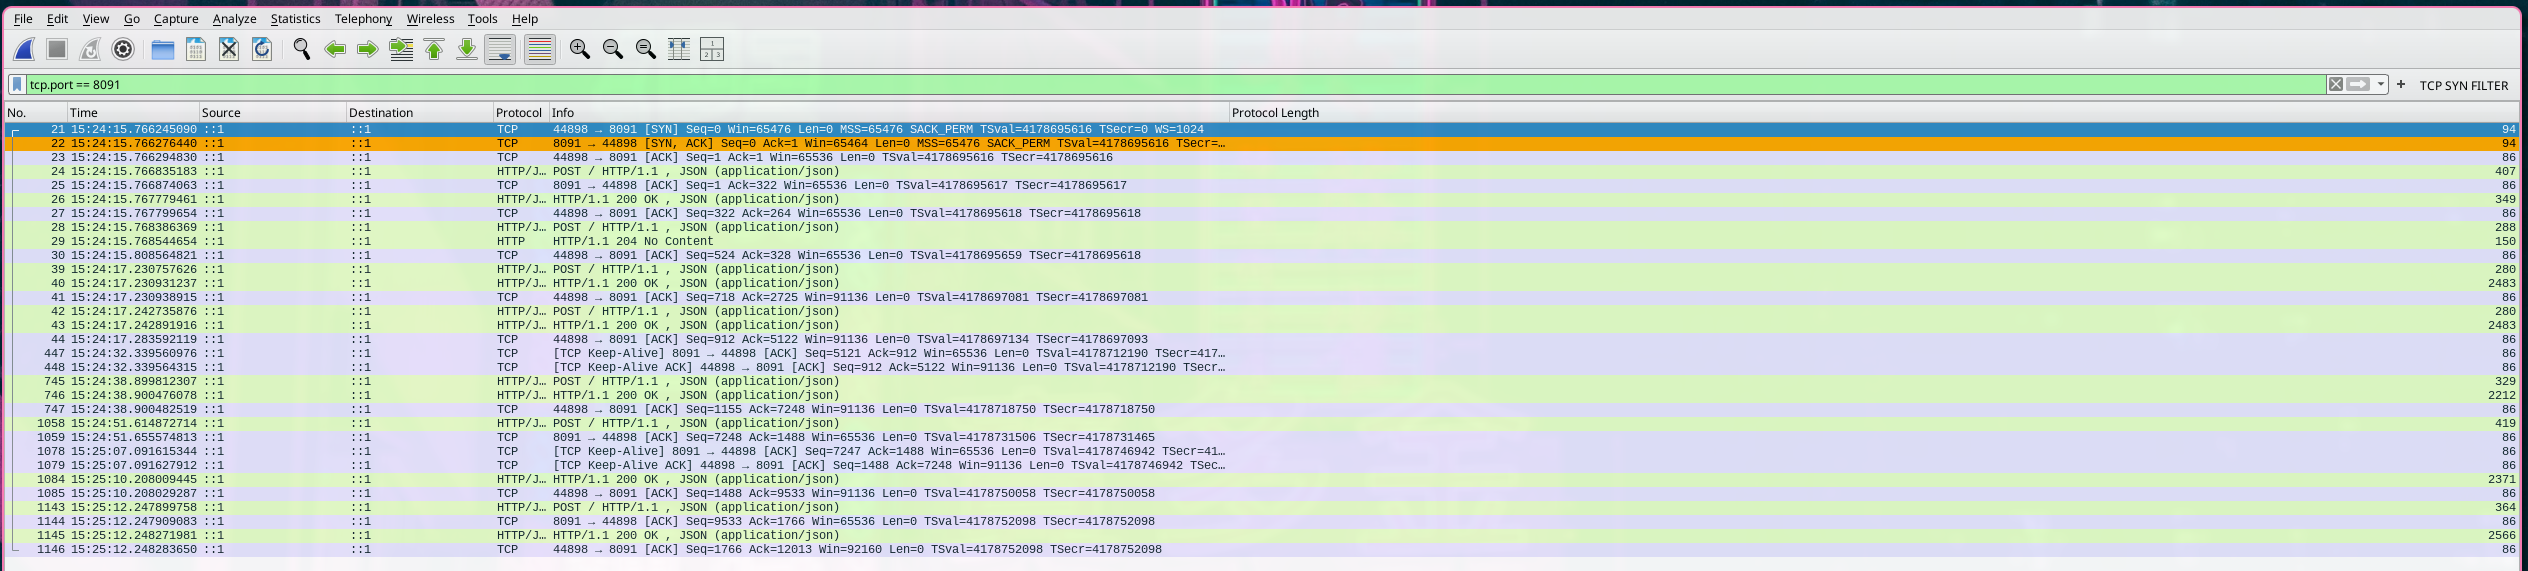
\includegraphics[width=0.95\textwidth]{figs/local-01-filtered-list.png}
% \caption{Captura local: paquetes filtrados con \texttt{tcp.port == 8091}.}
% \label{fig:local-filtered-list}
% \end{figure}
%
% \begin{figure}[ht]
% \centering
% \includegraphics[width=0.95\textwidth]{figs/local-02-loopback-header.png}
% \caption{Captura local: encabezado ``Null/Loopback'' --- sin trama
% Ethernet real, ya que el tráfico nunca sale de la interfaz \texttt{lo}.}
% \label{fig:local-loopback}
% \end{figure}
%
% \begin{figure}[ht]
% \centering
% 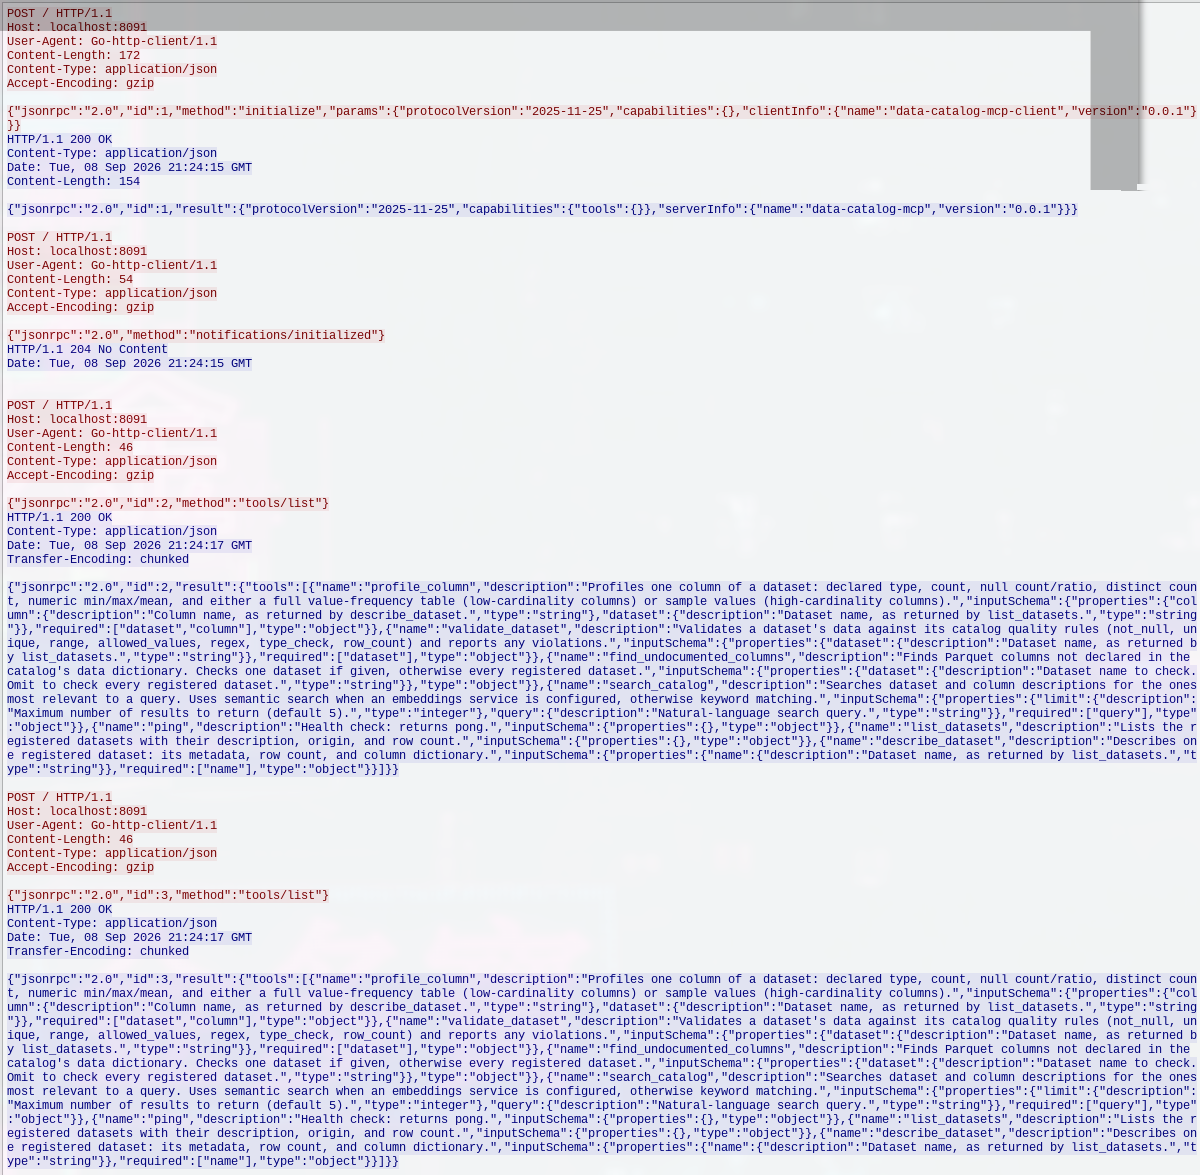
\includegraphics[width=0.95\textwidth]{figs/local-03-http-stream.png}
% \caption{Captura local: conversación completa vía Follow > HTTP Stream,
% mostrando en texto plano cada solicitud y respuesta JSON-RPC en orden.}
% \label{fig:local-http-stream}
% \end{figure}
%
% \begin{figure}[ht]
% \centering
% 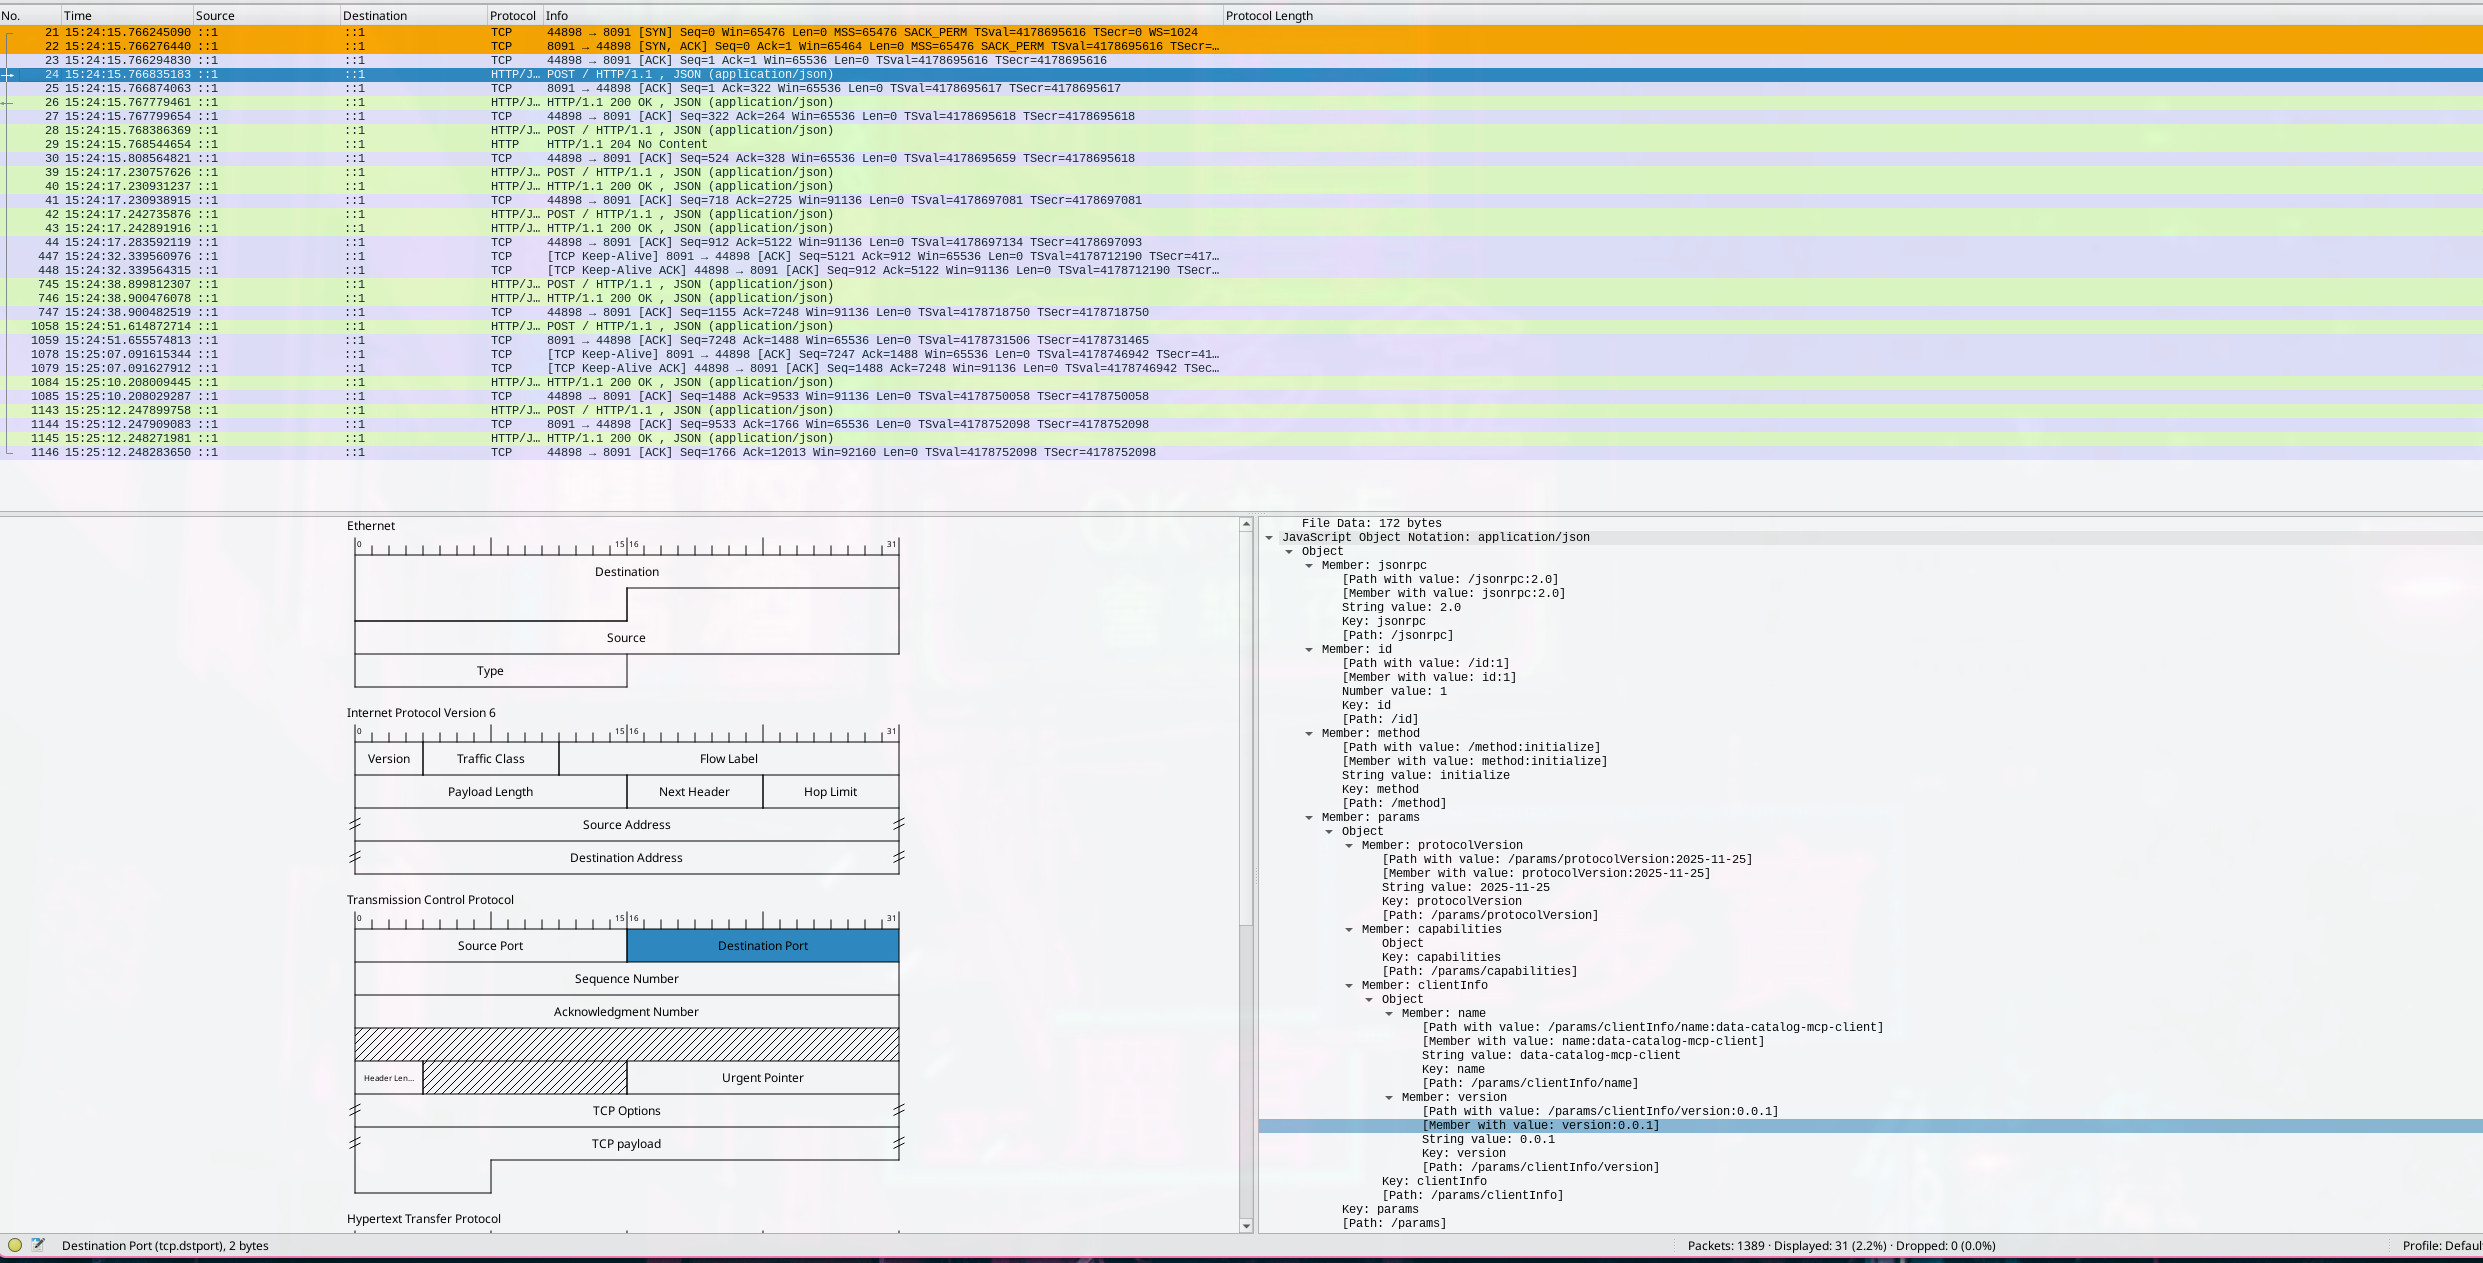
\includegraphics[width=0.95\textwidth]{figs/local-04-initialize-request.png}
% \caption{Captura local: cuerpo JSON de la solicitud \texttt{initialize}.}
% \label{fig:local-init-req}
% \end{figure}
%
% \begin{figure}[ht]
% \centering
% 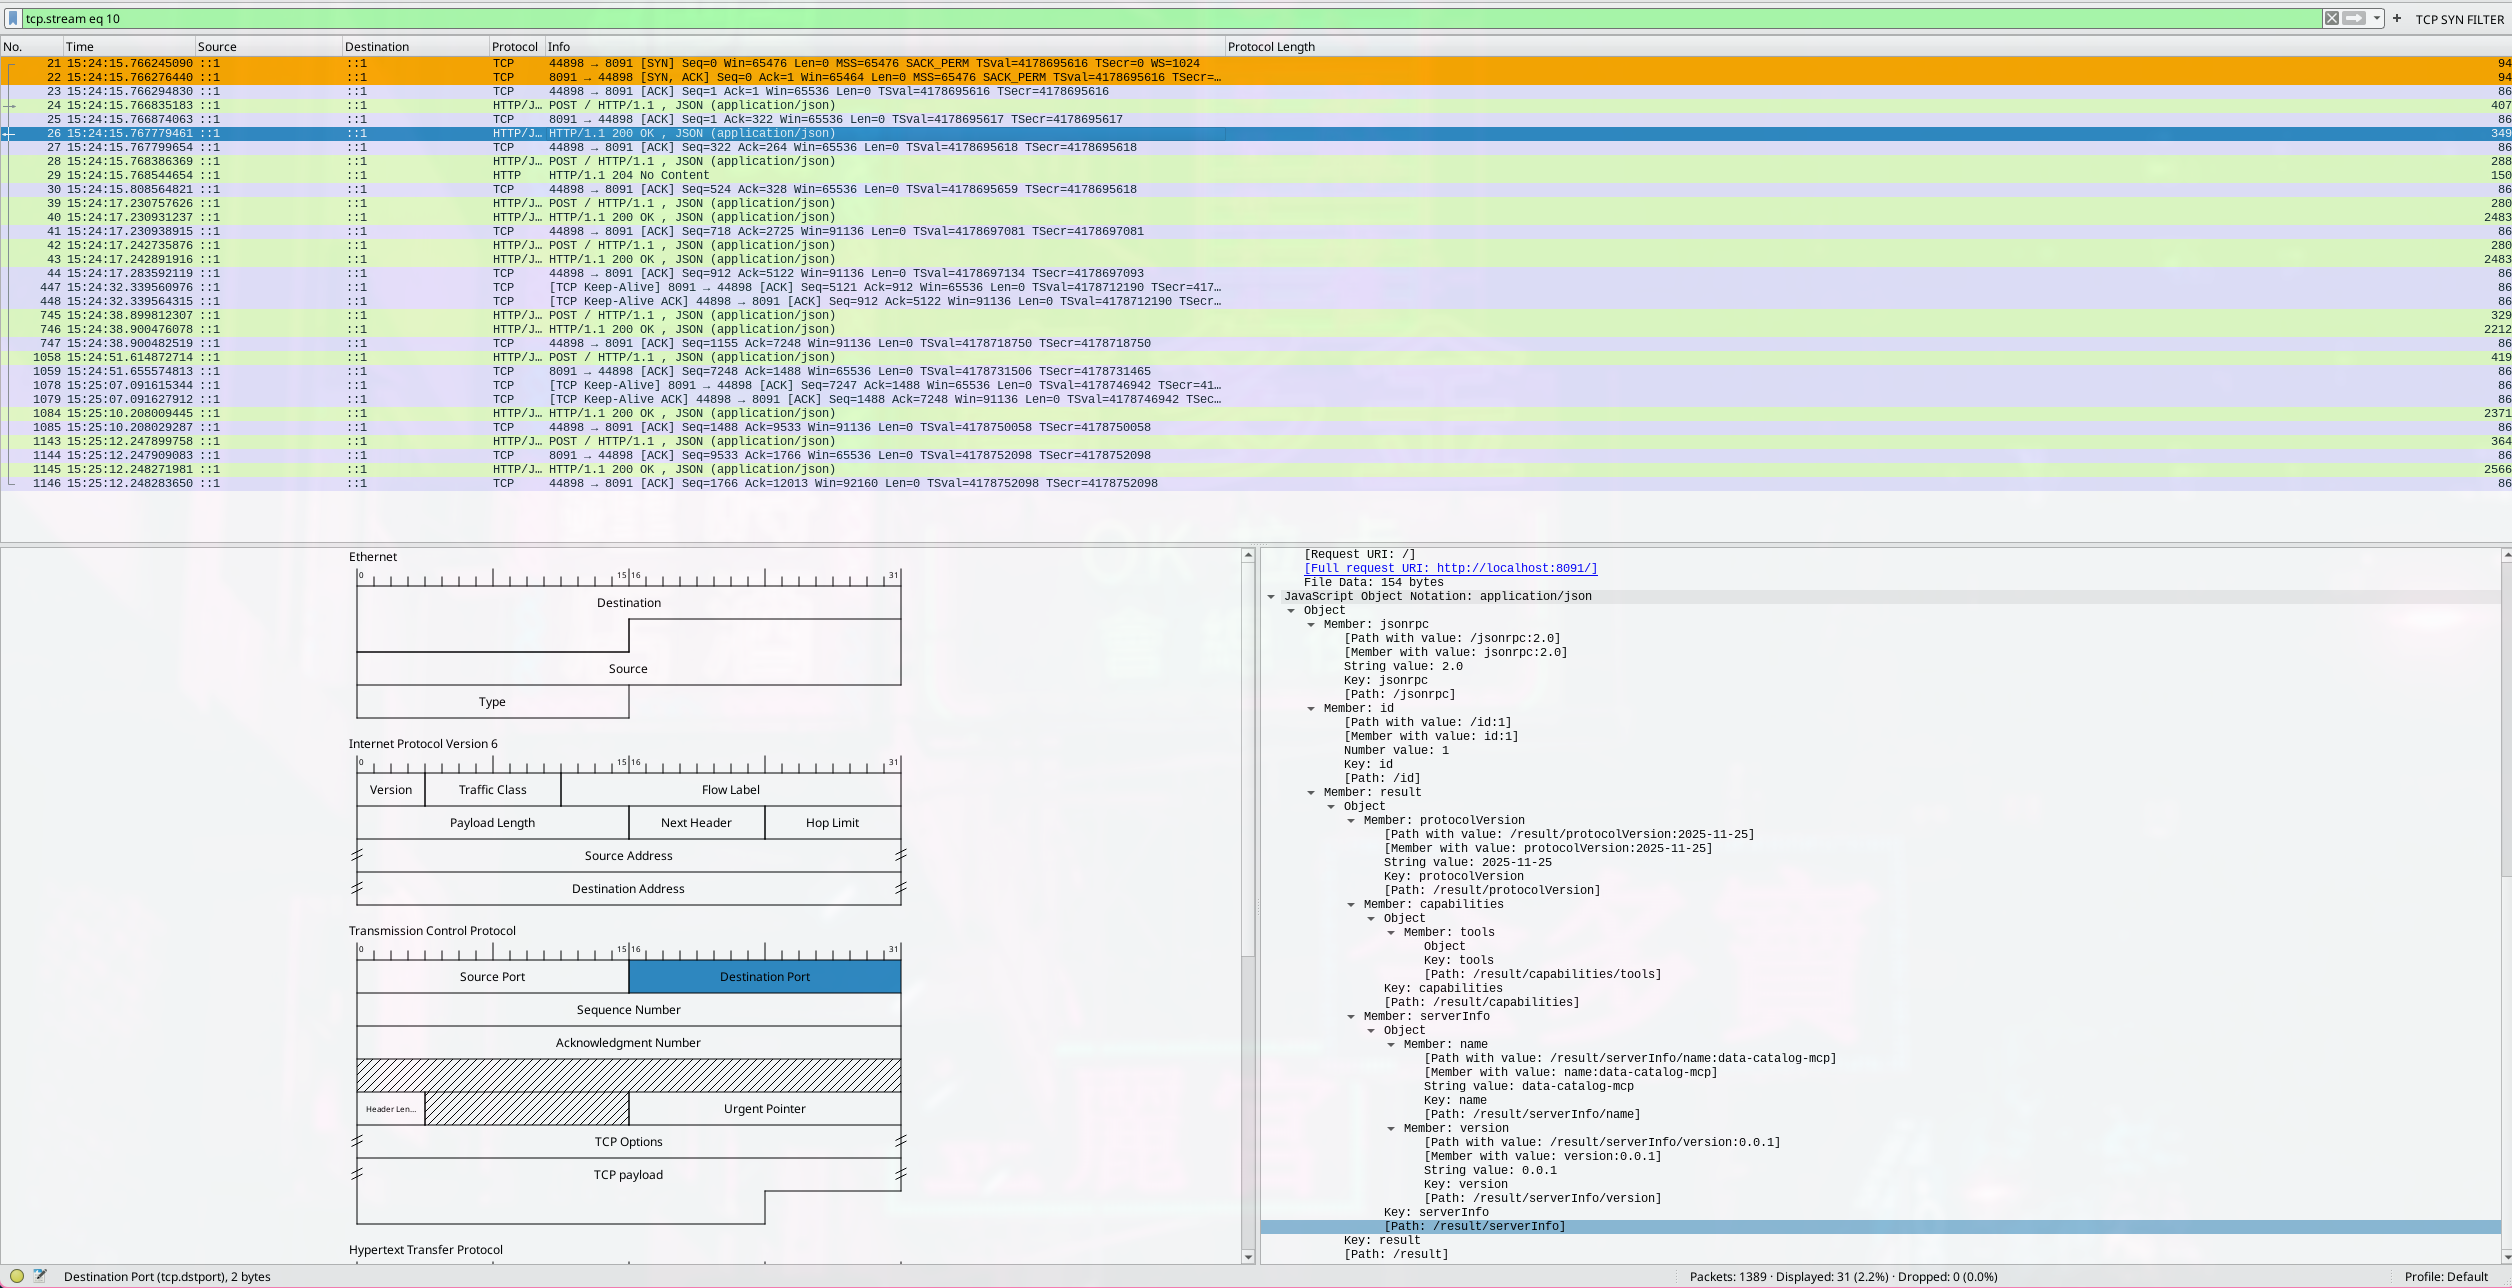
\includegraphics[width=0.95\textwidth]{figs/local-05-initialize-response.png}
% \caption{Captura local: respuesta a \texttt{initialize}, mismo \texttt{id}
% que la solicitud.}
% \label{fig:local-init-resp}
% \end{figure}
%
% \begin{figure}[ht]
% \centering
% 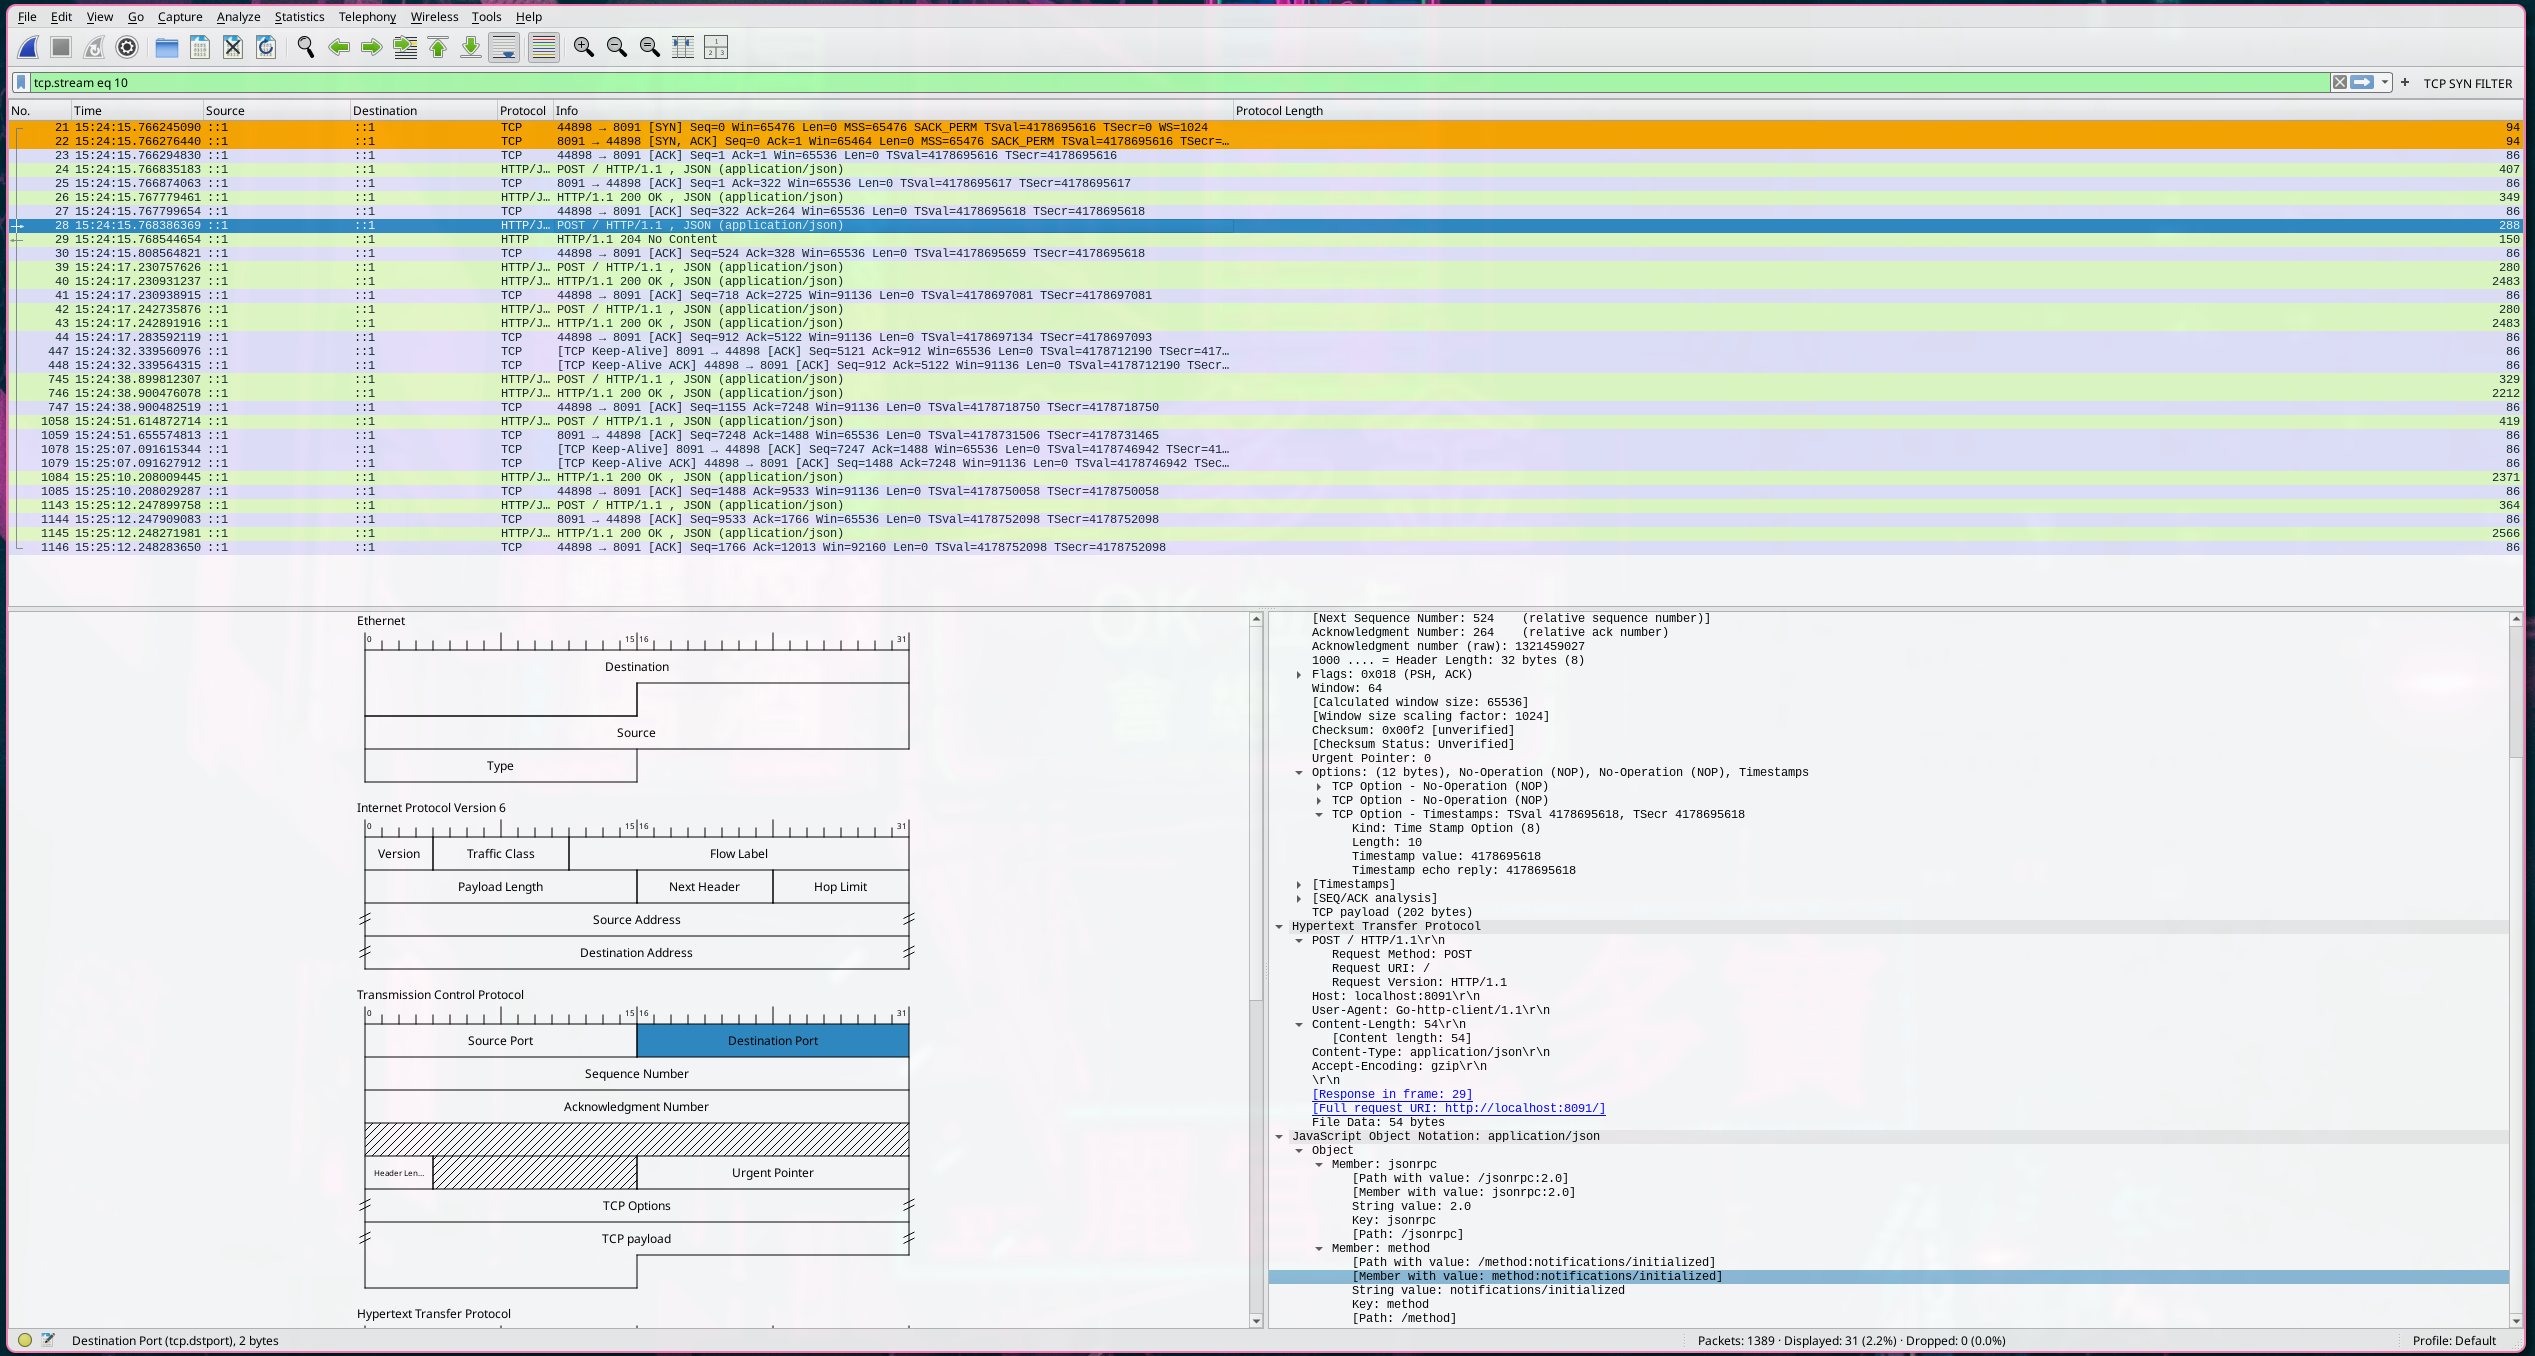
\includegraphics[width=0.95\textwidth]{figs/local-06-notification.png}
% \caption{Captura local: \texttt{notifications/initialized} --- nótese la
% ausencia del campo \texttt{id}, lo que la identifica como notificación.}
% \label{fig:local-notification}
% \end{figure}
%
% \begin{figure}[ht]
% \centering
% 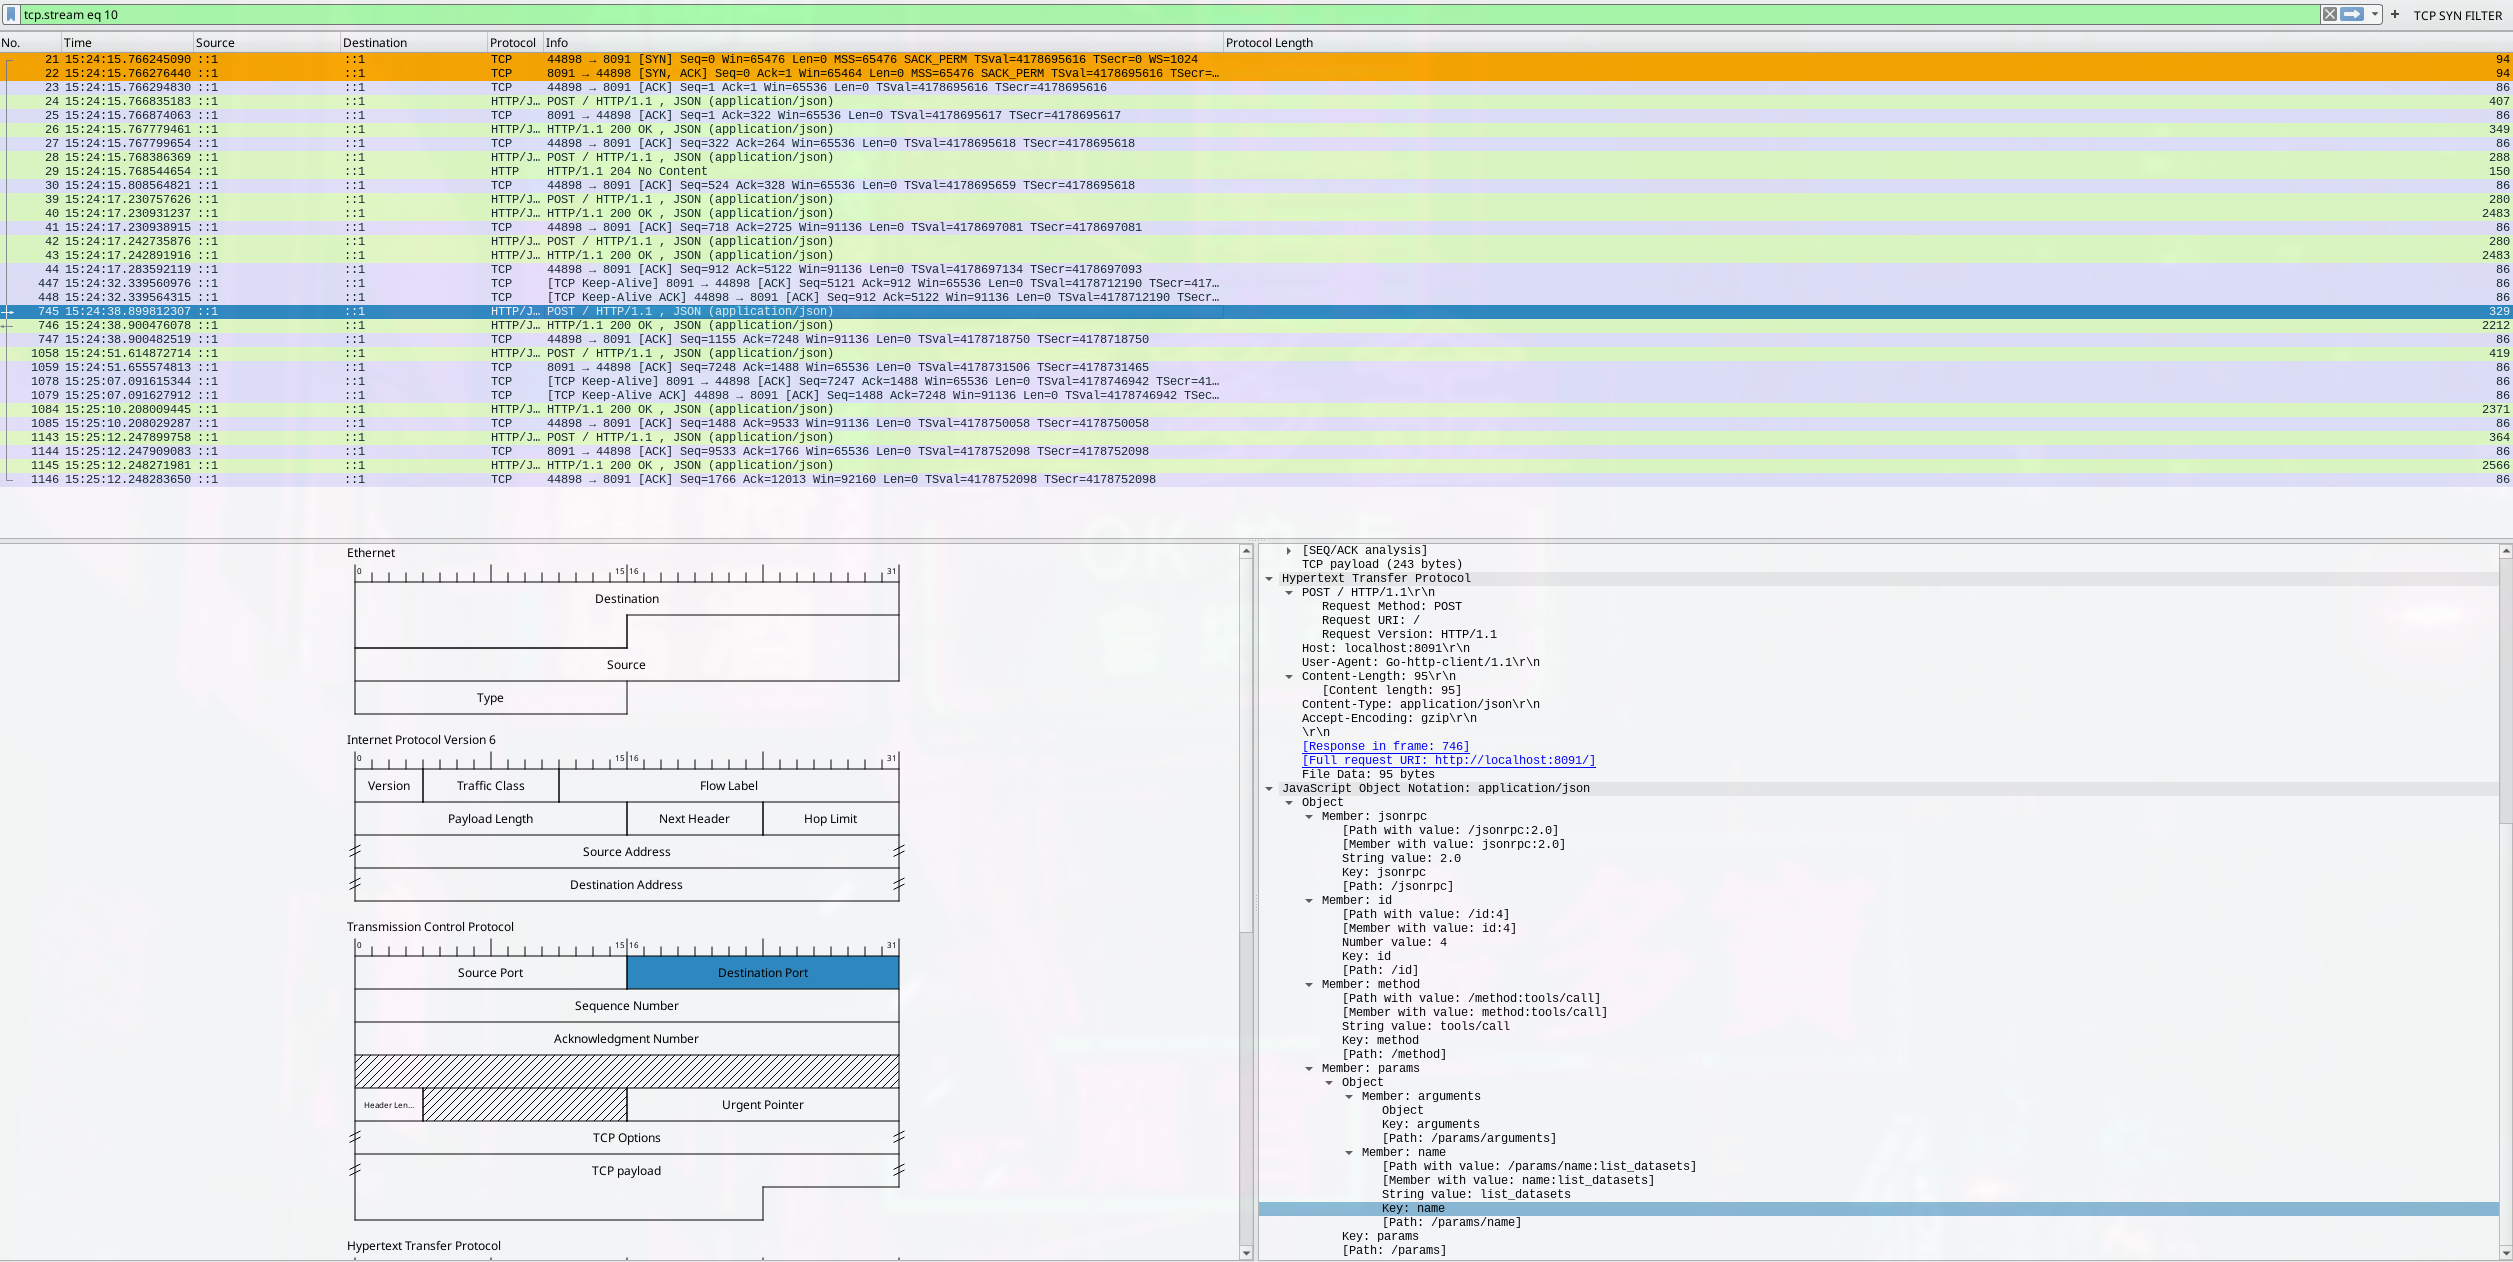
\includegraphics[width=0.95\textwidth]{figs/local-07-toolscall-request.png}
% \caption{Captura local: solicitud \texttt{tools/call}.}
% \label{fig:local-call-req}
% \end{figure}
%
% \begin{figure}[ht]
% \centering
% 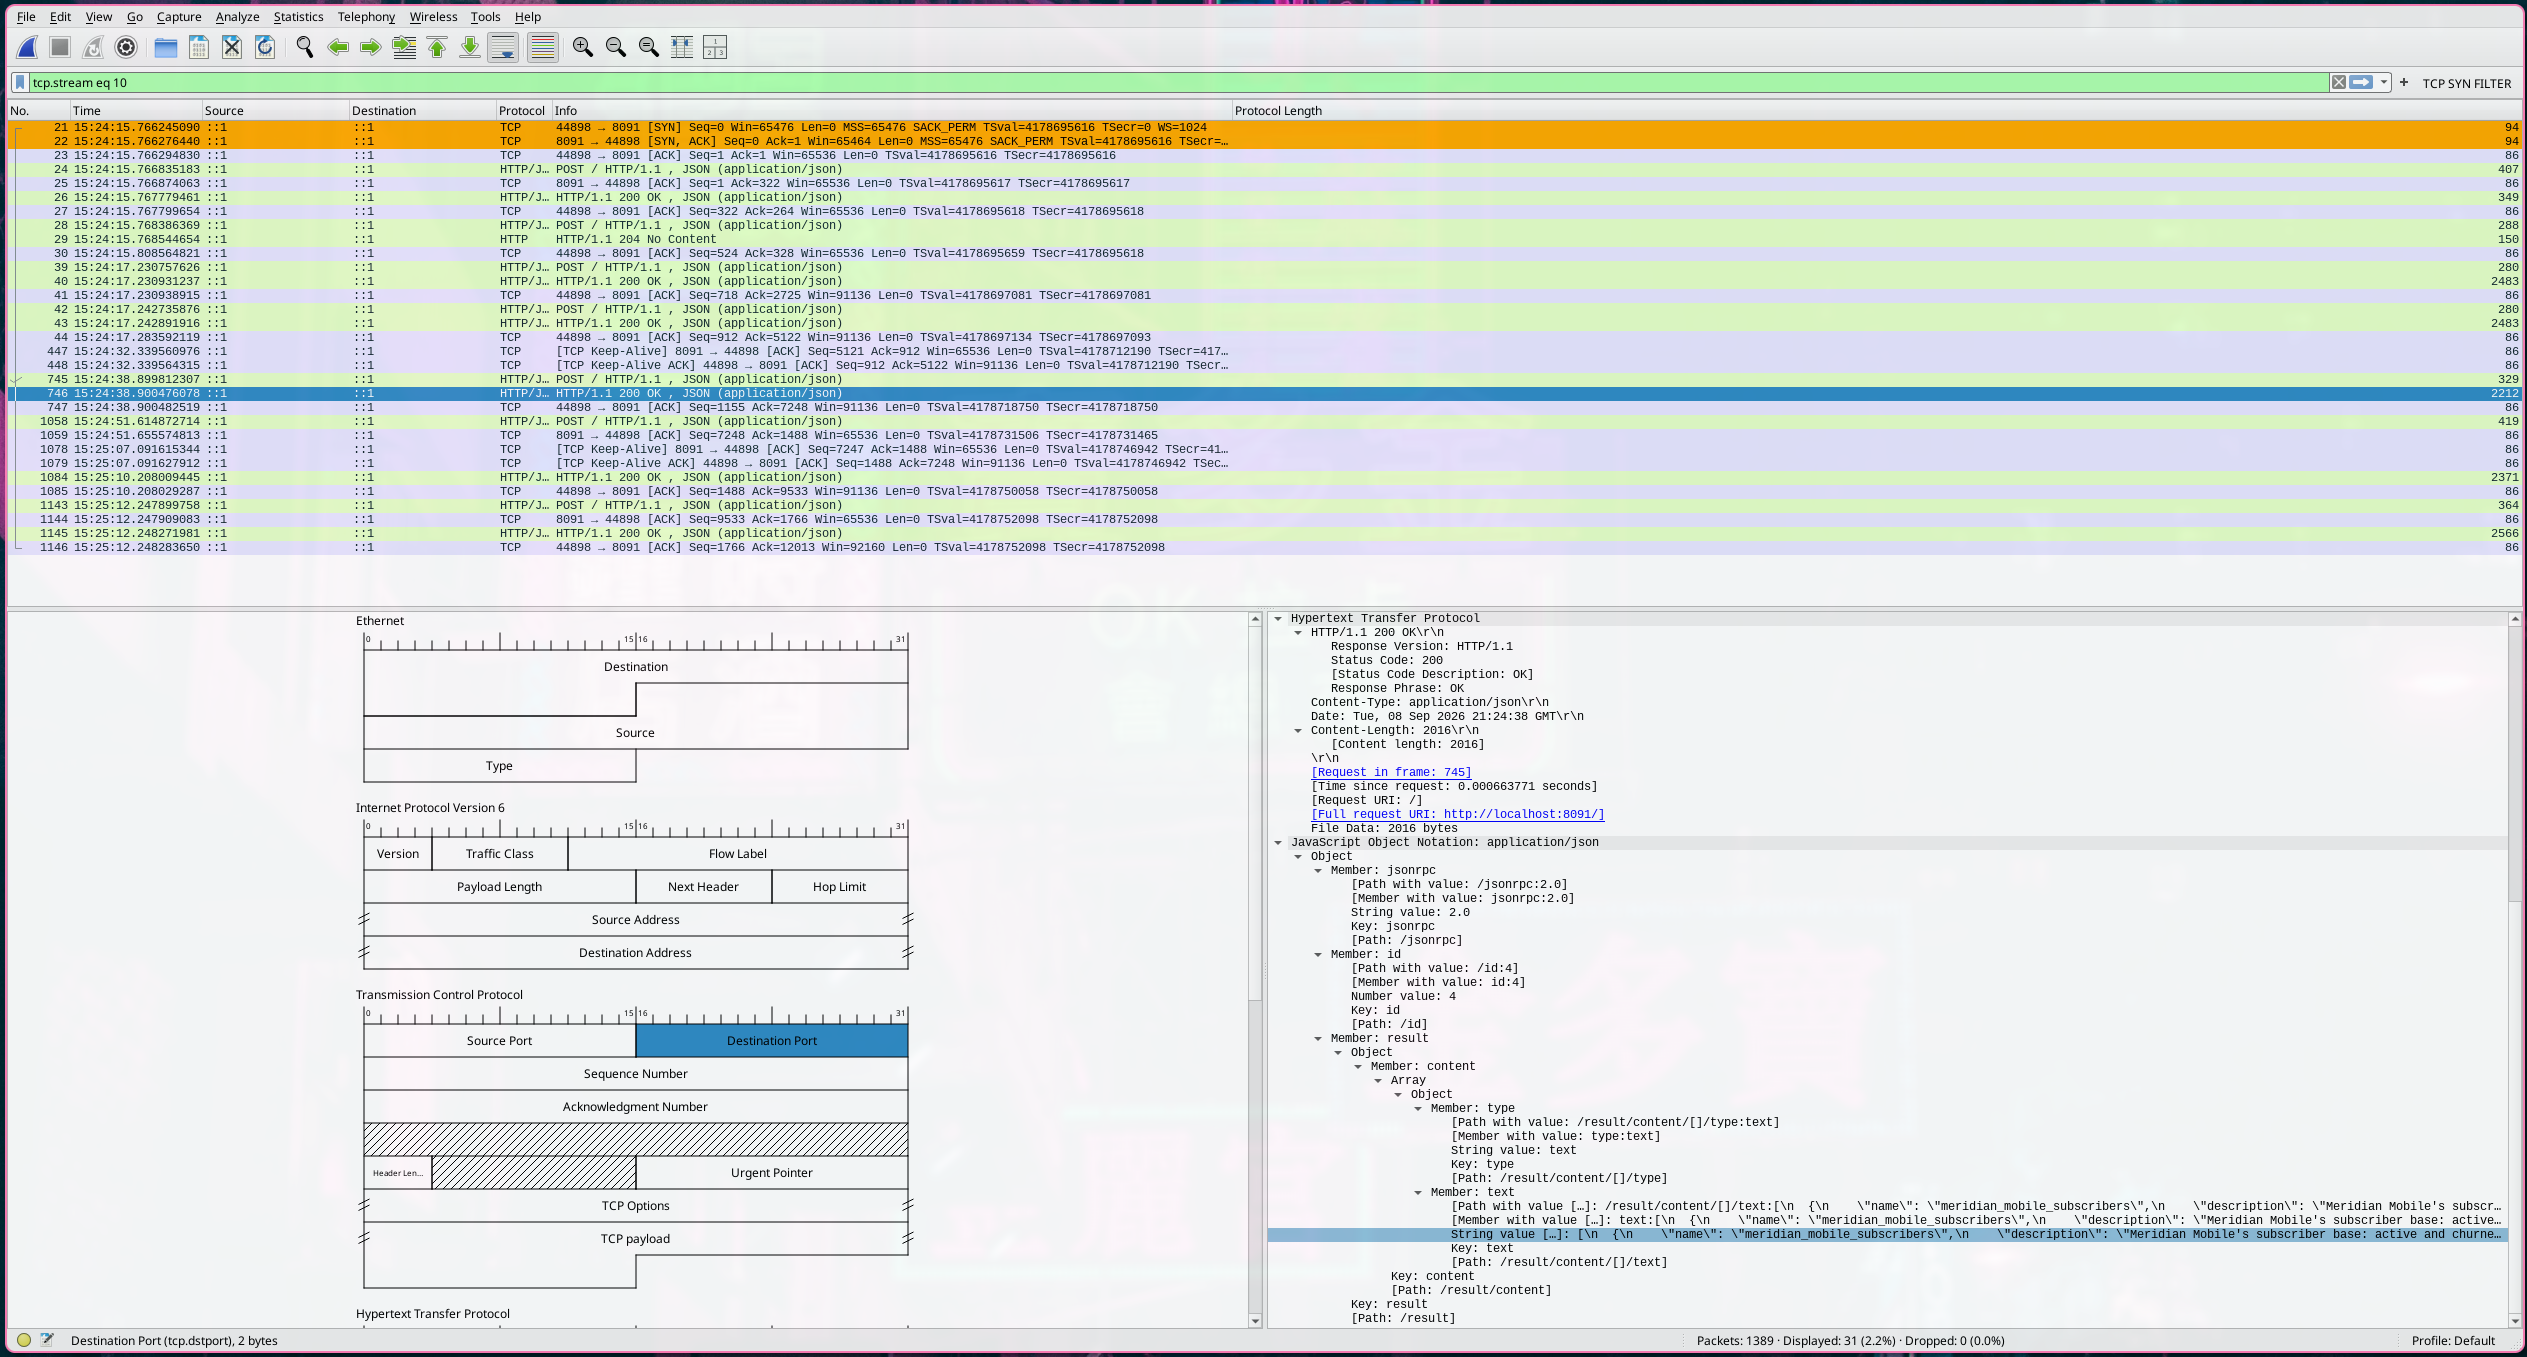
\includegraphics[width=0.95\textwidth]{figs/local-08-toolscall-response.png}
% \caption{Captura local: respuesta a la llamada de herramienta.}
% \label{fig:local-call-resp}
% \end{figure}

\subsection{Análisis por capa}
\label{sec:capas}

\paragraph{Capa de enlace.}
En la captura remota (Figura~\ref{fig:ip-layer}), Wireshark reporta un
encabezado \textbf{Ethernet II} real: dirección MAC origen
\code{84:01:12:d3:19:e9} (identificada por el fabricante como
\texttt{KaonGroup}, la interfaz de red local de la máquina que capturó el
tráfico) y dirección MAC destino \code{0e:62:e7:72:da:65}. Esta última
\emph{no} es la MAC del servidor de Cloud Run --- por diseño, una dirección
MAC nunca sobrevive más de un salto --- sino la del siguiente dispositivo en
la ruta (el gateway/router local). Esta es la única capa donde se opera
sobre un segmento físico compartido; a partir de la capa de red la
comunicación ya es de extremo a extremo lógico.

\paragraph{Capa de red.}
El mismo frame (Figura~\ref{fig:ip-layer}) muestra \textbf{IPv6}: dirección
origen \texttt{2800:98:1124:aa7::2} (la máquina cliente) y destino
\texttt{2600:1900:4243:200::} (la IP pública de Cloud Run, dentro del
bloque de Google Cloud). Wireshark resuelve esta última mediante su base de
datos GeoIP como ubicada en Estados Unidos --- una aproximación geográfica
basada en el bloque de direcciones, no necesariamente la región física
exacta (\texttt{northamerica-south1} en la consola de Cloud Run es la
región lógica del servicio, no implica que el bloque IP esté geolocalizado
con esa misma granularidad en bases de datos GeoIP de terceros). No se
observó fragmentación IP: todos los segmentos grandes se manejan a nivel de
TCP, no de IP.

\paragraph{Capa de transporte.}
Se observa el \textbf{three-way handshake} completo de TCP
(Figura~\ref{fig:tcp-handshake}): \texttt{SYN} (puerto efímero \texttt{43952}
del cliente $\to$ puerto \texttt{443} del servidor), \texttt{SYN, ACK} (el
paquete mostrado en detalle, con \texttt{Flags: 0x012}), y el \texttt{ACK}
final del cliente que completa la conexión. Sobre esa conexión TCP ya
establecida corre inmediatamente el \textbf{handshake TLS 1.3}
(Figura~\ref{fig:tls-handshake}): \texttt{Client Hello} --- que incluye el
campo SNI (\emph{Server Name Indication},
\texttt{data-catalog-mcp-53268160127.northamerica-\allowbreak
south1.run.app}), visible en claro pese a ser TLS, ya que el SNI viaja sin
cifrar para que el servidor sepa qué certificado presentar --- seguido de
\texttt{Server Hello, Change Cipher Spec}. A partir de ahí toda la
comunicación queda cifrada bajo TLS 1.3: sin acceso a las claves de sesión
(p.\,ej.\ vía \texttt{SSLKEYLOGFILE}), Wireshark solo puede mostrar
\textbf{Application Data} cifrada (Figura~\ref{fig:app-data}), no su
contenido. Esto confirma que la capa de transporte (TCP) entrega los datos
de forma confiable y ordenada independientemente de que estén cifrados o
no --- el cifrado es una responsabilidad de la capa superior (TLS, entre
transporte y aplicación), no de TCP en sí.

\paragraph{Capa de aplicación.}
Dentro de los registros \texttt{Application Data} de TLS, Wireshark
identifica el protocolo interno como \textbf{HTTP} (campo
\texttt{[Application Data Protocol: Hypertext Transfer Protocol]} en la
Figura~\ref{fig:app-data}), aunque no puede decodificar su contenido sin
las claves de sesión. Por diseño, el servidor MCP expone un único endpoint
HTTP (\code{POST /}, \code{Content-Type: application/json}) cuyo cuerpo es,
a su vez, un mensaje JSON-RPC --- es decir, JSON-RPC actúa como un
sub-protocolo de aplicación dentro de HTTP. En la captura local
(sin TLS, mismo servidor) este mismo intercambio es perfectamente legible;
la Tabla~\ref{tab:jsonrpc} y las figuras referenciadas en
\S\ref{sec:jsonrpc} muestran el contenido real de esos mensajes
\code{initialize}, \code{tools/list} y \code{tools/call}.

\begin{figure}[ht]
\centering
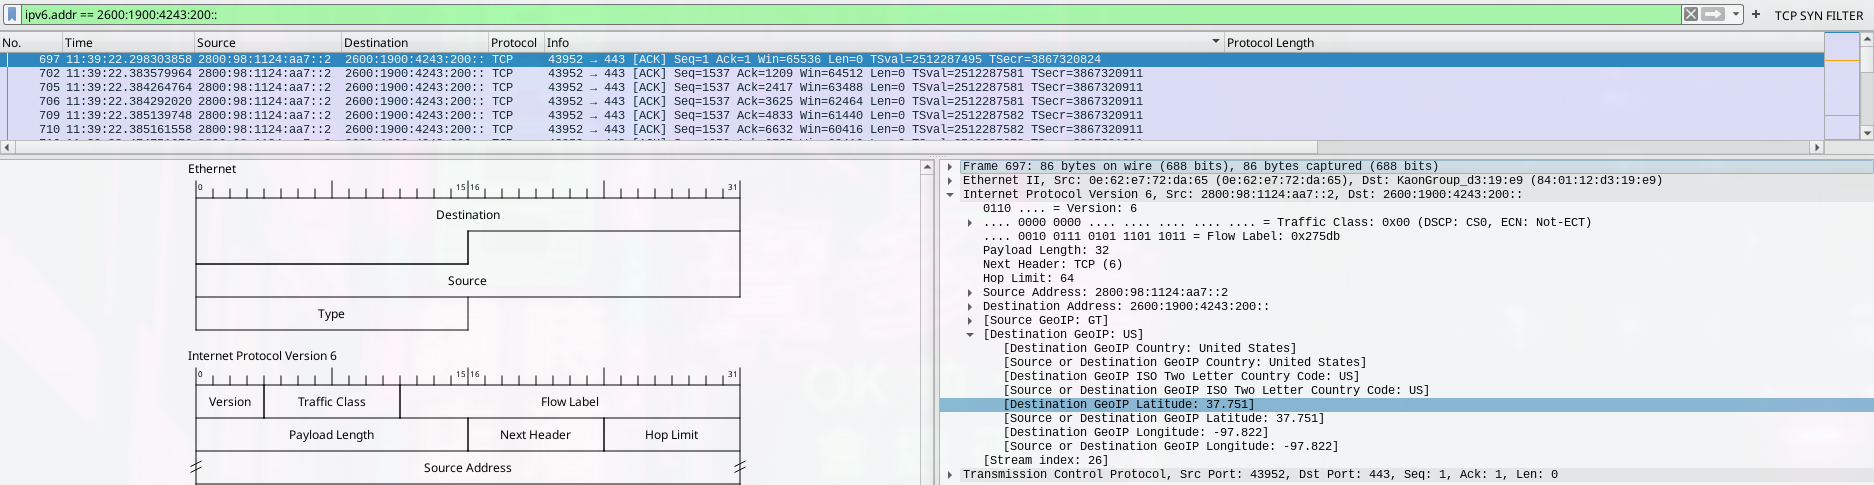
\includegraphics[width=0.95\textwidth]{figs/remote-05-ip-layer.png}
\caption{Captura remota: encabezado Ethernet II (capa de enlace) e IPv6
(capa de red) de un paquete ACK del handshake TCP contra Cloud Run.}
\label{fig:ip-layer}
\end{figure}

\begin{figure}[ht]
\centering
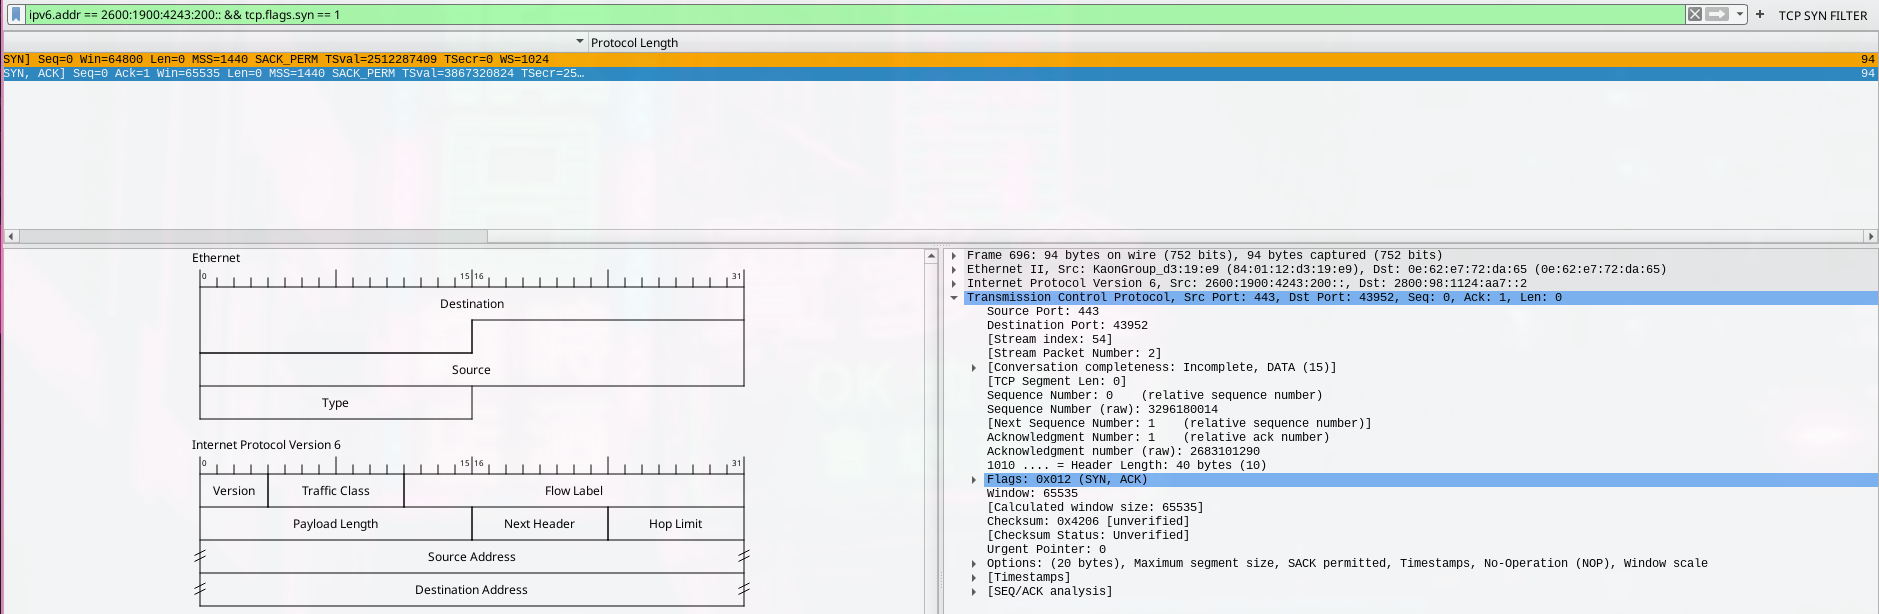
\includegraphics[width=0.95\textwidth]{figs/remote-02-tcp-handshake.png}
\caption{Captura remota: three-way handshake TCP (\texttt{tcp.flags.syn==1}),
con el paquete \texttt{SYN, ACK} expandido mostrando puertos y flags.}
\label{fig:tcp-handshake}
\end{figure}

\begin{figure}[ht]
\centering
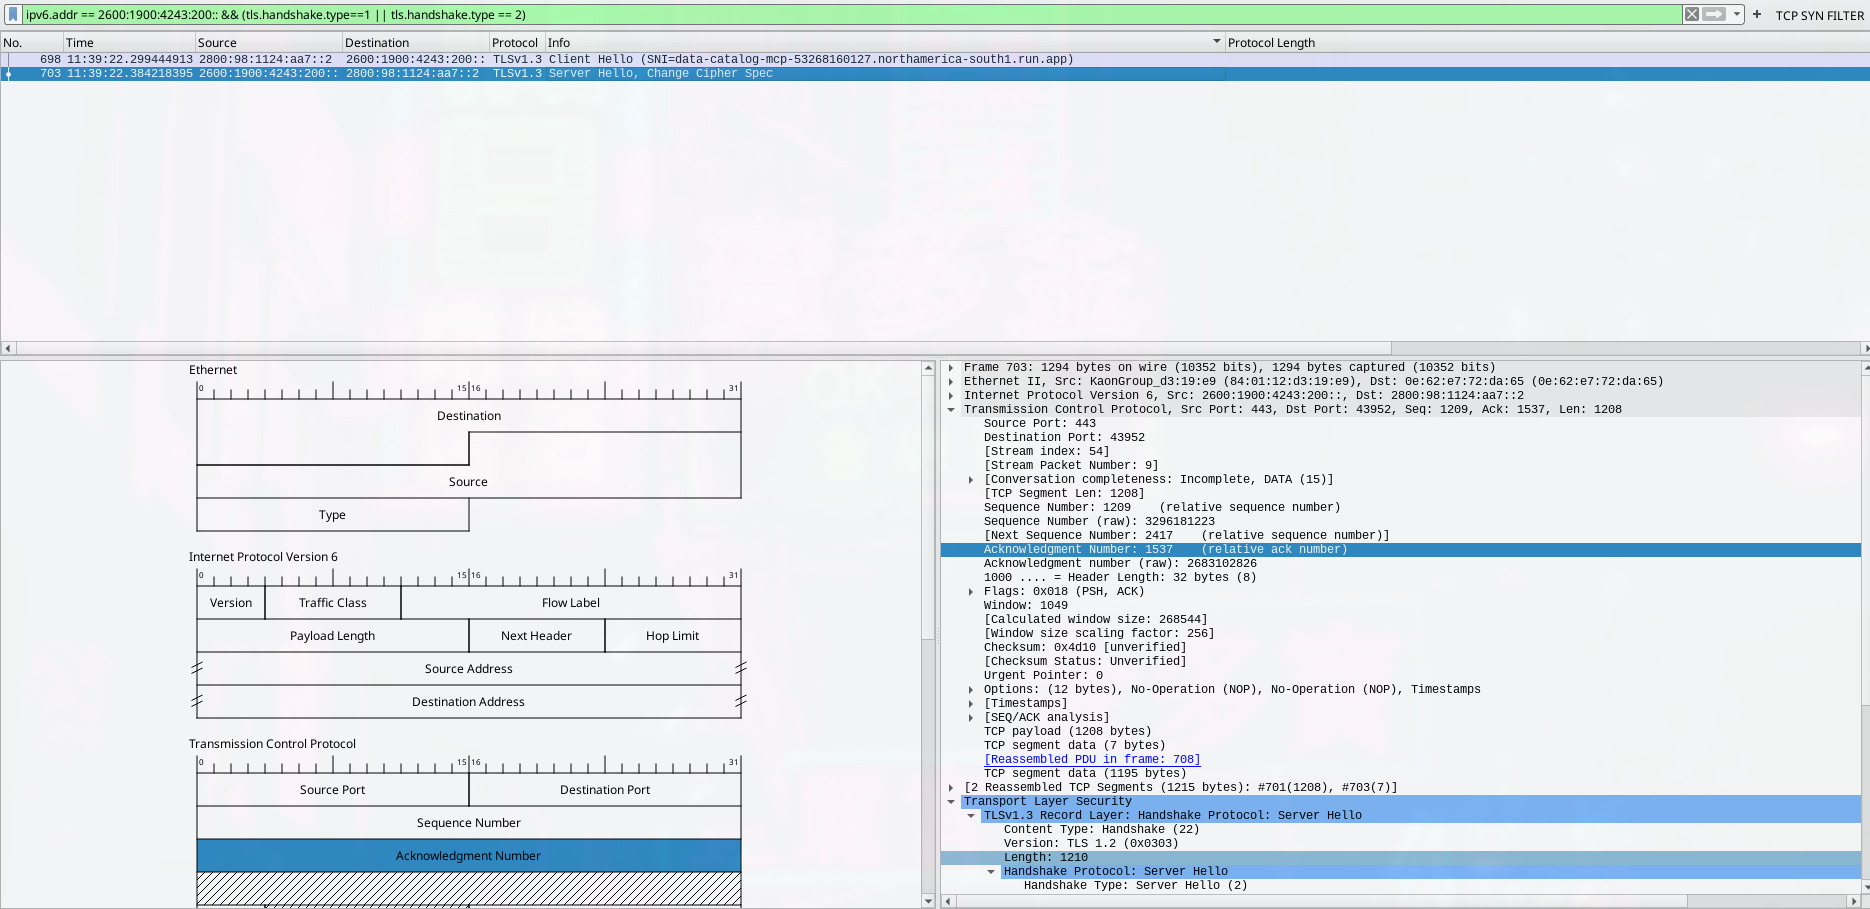
\includegraphics[width=0.95\textwidth]{figs/remote-03-tls-handshake.png}
\caption{Captura remota: handshake TLS 1.3 (\texttt{Client Hello} con SNI,
\texttt{Server Hello, Change Cipher Spec}).}
\label{fig:tls-handshake}
\end{figure}

\begin{figure}[ht]
\centering
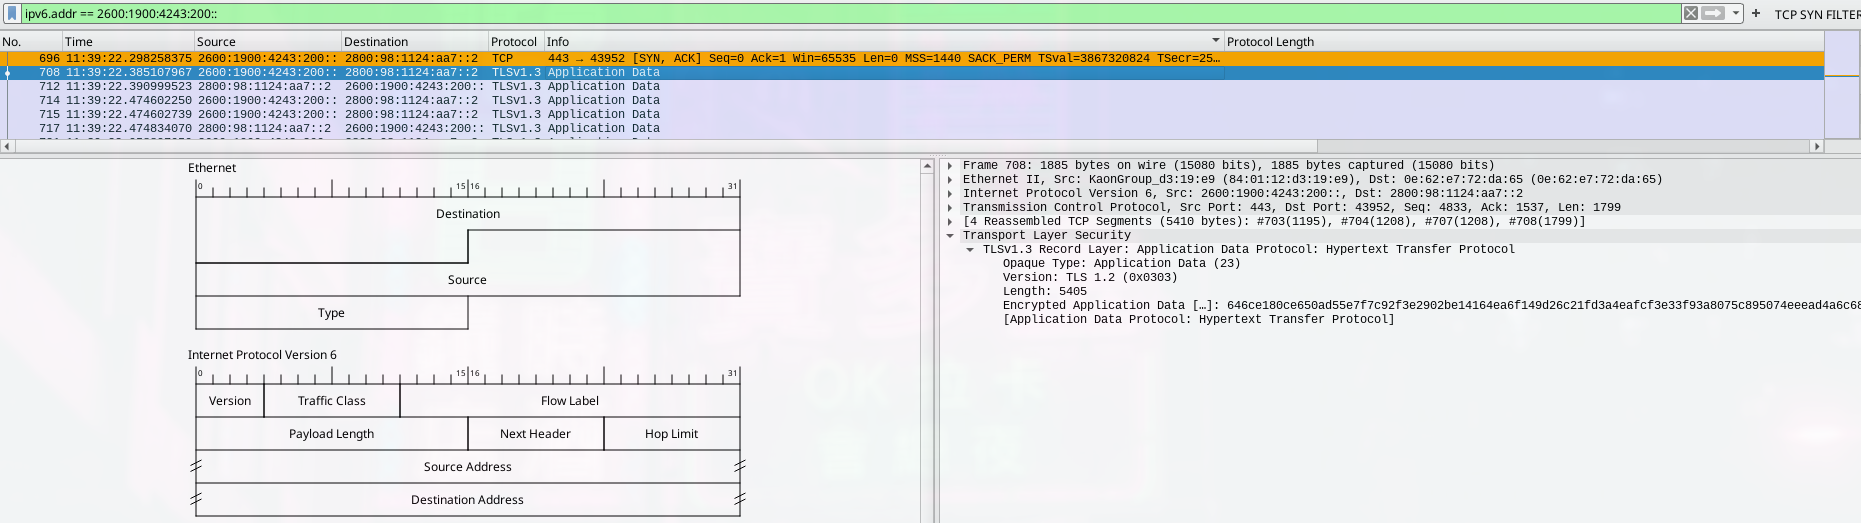
\includegraphics[width=0.95\textwidth]{figs/remote-04-app-data-encrypted.png}
\caption{Captura remota: registro TLS de \texttt{Application Data} cifrado,
identificado como HTTP a nivel de protocolo pero ilegible sin las claves de
sesión.}
\label{fig:app-data}
\end{figure}

\section{Conclusiones y comentario sobre el proyecto}

% TODO: características implementadas, dificultades encontradas (ej. framing
% de JSON-RPC a mano, manejo de stdio vs HTTP, despliegue en Cloud Run,
% embeddings y su degradación a búsqueda por palabra clave), y lecciones
% aprendidas sobre el protocolo MCP y su relación con JSON-RPC/HTTP/TCP/IP.

\end{document}
